\documentclass[10pt,aspectratio=169]{beamer}
\usepackage[T1]{fontenc}
\usepackage{lmodern,amsmath,amssymb,booktabs,array,adjustbox,graphicx}
\graphicspath{{../figures/}}
\definecolor{Ink}{HTML}{172B3A}
\definecolor{Accent}{HTML}{007F79}
\definecolor{Muted}{HTML}{556570}
\definecolor{Warn}{HTML}{B5532B}
\setbeamercolor{normal text}{fg=Ink,bg=white}
\setbeamercolor{structure}{fg=Accent}
\setbeamercolor{frametitle}{fg=Ink,bg=white}
\setbeamercolor{itemize item}{fg=Accent}
\setbeamerfont{frametitle}{size=\Large,series=\bfseries}
\setbeamertemplate{navigation symbols}{}
\setbeamertemplate{itemize item}{\small\textbullet}
\setbeamersize{text margin left=9mm,text margin right=9mm}
\setbeamertemplate{footline}{\hfill\textcolor{Muted}{\scriptsize\insertframenumber/\inserttotalframenumber}\hspace{9mm}\vspace{3mm}}
\setbeamertemplate{frametitle}{\vspace{3mm}\insertframetitle\par\vspace{1.5mm}\textcolor{Accent}{\rule{\textwidth}{0.5pt}}}
\setlength{\parskip}{1pt}
\newcommand{\key}[1]{\textcolor{Accent}{\textbf{#1}}}
\newcommand{\fn}[1]{\textcolor{Muted}{\scriptsize #1}}
\hypersetup{pdftitle={DIALS: Learning How to Combine Bundle Evidence},colorlinks=true,urlcolor=Accent}
\begin{document}

% ------------------------------------------------------------------ 1
\begin{frame}{DIALS: learning how to combine bundle evidence}
\vspace{3mm}
\key{Task:} given some items of a bundle, rank the whole catalogue for the missing ones.\par
\vspace{4mm}
\key{DIALS:} content, label and co-occurrence terms, each learned, combined by a per-query gate; 41.6k parameters, one configuration on 8 datasets.\par
\vspace{5mm}
\key{Questions this talk answers:}
\begin{enumerate}\setlength\itemsep{4pt}
\item Combining history and descriptive evidence has been done before. What is different here?
\item Is it just an ensemble of existing scorers?
\item Does a 41.6k-parameter model have practical value against CLHE or RaMen?
\item Where does it not work?
\end{enumerate}
\end{frame}

% ------------------------------------------------------------------ bridge from BundleFuse
\begin{frame}{From BundleFuse to DIALS}
\small
\key{BundleFuse (presented last time):} no trained scorer. Standardized evidence scores, weights chosen on validation, a frequency fallback $\frac{f_c}{f_c+\kappa}$. It beat published RaMen on POG and Spotify (+45\% and +43\% Recall@20).\par
\vspace{1.5mm}
\key{What it showed:} how evidence is combined matters more than model size; history and attributes are both needed.\par
\vspace{1.5mm}
\renewcommand{\arraystretch}{1.1}
\begin{adjustbox}{max width=\textwidth}\begin{tabular}{@{}>{\raggedright\arraybackslash}p{0.29\textwidth}>{\raggedright\arraybackslash}p{0.31\textwidth}>{\raggedright\arraybackslash}p{0.34\textwidth}@{}}
\toprule
\textbf{BundleFuse, fixed by hand} & \textbf{What that could not do} & \textbf{DIALS, learned}\\\midrule
One weight per source, per dataset & change the mix from query to query & a gate $w(S)$ per query\\
Fallback $\frac{f_c}{f_c+\kappa}$ & adapt to how much history the seeds have & gate inputs plus a prior $\rho(f_c)$\\
Category evidence as similarity & learn ``avoid the seed's category'' & signed $\delta_l$ plus a label relation $P_lM_lQ_l^\top$\\
Recipe picked per dataset & one method for every dataset & one configuration on 8 datasets\\\bottomrule
\end{tabular}\end{adjustbox}\par
\vspace{1.5mm}
\key{DIALS keeps BundleFuse's evidence and learns its hand-set choices, with 41.6k parameters.}
\end{frame}

% ------------------------------------------------------------------ why DIALS
\begin{frame}{Why DIALS: what it offers}
\key{Bundle completion that still works when the items have no purchase history, at a fraction of the size of neural models.}\par
\vspace{3mm}
\small
\begin{itemize}\setlength\itemsep{4pt}
\item \key{Works without history.} On POG 96\% of test queries have no co-occurrence evidence; there DIALS scores NDCG@20 .019 against CLHE's .005. On Spotify\_sparse targets with no history: .263 against .003.
\item \key{More accurate on identical splits and features.} Ahead of CLHE on all 6 datasets where it was rerun, and of RaMen on the 3 where it was: +.014 to +.197 NDCG@20, all $p=.002$.
\item \key{Cheap to run.} 41.6k parameters (18--1,350$\times$ fewer), none per item; trains on CPU in 12--15 min on POG; a new item is scored on day one, without retraining.
\item \key{Readable.} Every score splits into named terms and gate weights; the learned sign of the category term flips between domains (avoid the seed's category on fashion, prefer the same artist on music).
\end{itemize}
\vspace{2mm}
\key{Where it stops:} on warm grocery baskets (Dunnhumby) it ties the best simple baseline. The case for DIALS is new, sparse or changing catalogues.
\end{frame}

% ------------------------------------------------------------------ 2
\begin{frame}{The task and three kinds of evidence}
\[
 S=\{\text{seed items}\}\;\longrightarrow\;\operatorname{TopK}_{c\notin S}\; s(c\mid S)
\]
\vspace{2mm}
Three kinds of evidence about a candidate $c$:\par
\vspace{3mm}
\renewcommand{\arraystretch}{1.3}
\begin{adjustbox}{max width=\textwidth}\begin{tabular}{@{}>{\raggedright\arraybackslash}p{0.26\textwidth}>{\raggedright\arraybackslash}p{0.38\textwidth}>{\raggedright\arraybackslash}p{0.30\textwidth}@{}}
\toprule
\textbf{Evidence} & \textbf{Question it answers} & \textbf{Fails when}\\\midrule
History (co-occurrence) & Was $c$ bundled with these seeds? & $c$ or the seeds are rare or new\\
Content (features) & Does $c$ look like what goes with them? & resemblance $\neq$ compatibility\\
Labels (category, artist) & Does $c$'s category go with theirs? & categories too coarse\\\bottomrule
\end{tabular}\end{adjustbox}\par
\vspace{5mm}
\key{The question is not whether to use all three, but how much to trust each one, for each query.}
\end{frame}

% ------------------------------------------------------------------ 3
\begin{frame}{Is combining history and description new? No}
\renewcommand{\arraystretch}{1.25}\small
\begin{adjustbox}{max width=\textwidth}\begin{tabular}{@{}>{\raggedright\arraybackslash}p{0.21\textwidth}>{\raggedright\arraybackslash}p{0.20\textwidth}>{\raggedright\arraybackslash}p{0.08\textwidth}>{\raggedright\arraybackslash}p{0.45\textwidth}@{}}
\toprule
\textbf{Method} & \textbf{History} & \textbf{Labels} & \textbf{How the evidence is combined}\\\midrule
Hybrid CF (content + ItemKNN) & co-occurrence & no & fixed weighted sum, one weight per dataset\\
CLHE (WSDM'24) & user--item LightGCN view & no & attention fuses ID, multimodal and CF views into \key{one item vector}\\
RaMen (ECAI'25) & item--item graph, hypergraph & no & fixed mixing constants, then \key{one item vector}\\
\key{DIALS} & bundle counts & yes & separate terms, \key{weights learned per query}, label relation learned\\\bottomrule
\end{tabular}\end{adjustbox}\par
\vspace{2mm}
\key{What is different is where and how the evidence is combined, not that it is.}
\end{frame}

% ------------------------------------------------------------------ 4
\begin{frame}{What is different: separate terms, not one item vector}
\small
\begin{columns}[T,onlytextwidth]
\begin{column}{0.48\textwidth}
\key{Early fusion} (CLHE, RaMen)\par\vspace{1mm}
$\;s(c\mid S)=\mathrm{enc}(S)^\top v_c,\quad v_c=\mathrm{fuse}(\text{ID},\text{content},\text{graph})$\par
\vspace{1mm}
Evidence is mixed before scoring, so no query can say ``these seeds have no history, trust content''.
\end{column}
\begin{column}{0.48\textwidth}
\key{Late fusion with a gate} (DIALS)\par\vspace{1mm}
$\;s=w_C(S)\,C+\sum_l w_l(S)\,L_l+w_G(S)\,G$\par
\vspace{1mm}
Each evidence type keeps its own score, so seeds with no history still get content and label evidence.
\end{column}
\end{columns}
\vspace{2mm}
\textbf{Spotify\_sparse, test NDCG@20 by share of targets with any co-occurring seed:}\par\vspace{1mm}
\centering\renewcommand{\arraystretch}{1.05}
\begin{adjustbox}{max width=\textwidth}\begin{tabular}{lrrrrr}\toprule
Share with history & 0\% & (0, 25\%) & [25, 50\%) & [50, 75\%) & [75, 100\%]\\
Queries & 132 & 274 & 540 & 743 & 808\\\midrule
CLHE & .003 & .022 & .051 & .104 & .219\\
\key{DIALS} & \textbf{.263} & \textbf{.296} & \textbf{.218} & \textbf{.222} & \textbf{.298}\\
DIALS, co-occurrence switched off & .272 & .305 & .225 & .213 & .254\\
\key{Gain from co-occurrence} & $-$.009 & $-$.009 & $-$.007 & +.009 & \textbf{+.044}\\\bottomrule
\end{tabular}\end{adjustbox}\par
\raggedright\vspace{1mm}
\fn{Columns hold different queries: compare within a column. Co-occurrence switched off at inference, weights kept, 3 seeds; per-column differences not tested. The gate sees seeds, not which targets have history, so where few do, co-occurrence promotes wrong items.}
\end{frame}

% ------------------------------------------------------------------ 5
\begin{frame}{What is different: labels, which CLHE and RaMen leave out}
\textbf{Simple label-aware rules} (same label, label-to-label transition, blended with ItemKNN and content; tuned on validation)\par
\vspace{3mm}
\centering\renewcommand{\arraystretch}{1.4}
\begin{adjustbox}{max width=\textwidth}\begin{tabular}{lrrrr}\toprule
Test NDCG@20 (clean) & POG\_DENSE & POG & Spotify\_sparse & Spotify\\\midrule
CLHE (rerun, same features) & .248 & .0172 & .115 & .179$^\dagger$\\
Best label-aware simple rule & .249 & .0234 & .205 & .247\\
\key{DIALS} & \textbf{.280} & \textbf{.0313} & \textbf{.256} & \textbf{.282}\\
$\Delta$ DIALS $-$ best rule & +.031 & +.008 & +.051 & +.036\\
\quad 95\% CI & [.028, .034] & [.006, .010] & [.046, .056] & [.031, .040]\\\bottomrule
\end{tabular}\end{adjustbox}\par
\raggedright\vspace{3mm}
\fn{Holm over 8 tests (N and R): all $p=.0008$. $^\dagger$1 of 3 CLHE seeds finished on Spotify, all queries.}\par
\vspace{3mm}
\key{Labels alone beat CLHE; DIALS still beats the best rule that uses them.}
\end{frame}

% ------------------------------------------------------------------ 5b


% ------------------------------------------------------------------ 6
\begin{frame}{Each design choice, and the evidence for it}
\renewcommand{\arraystretch}{1.12}\small
\begin{adjustbox}{max width=\textwidth}\begin{tabular}{@{}>{\raggedright\arraybackslash}p{0.25\textwidth}>{\raggedright\arraybackslash}p{0.22\textwidth}>{\raggedright\arraybackslash}p{0.47\textwidth}@{}}
\toprule
\textbf{Choice} & \textbf{Simpler alternative} & \textbf{Evidence}\\\midrule
Separate learned terms & one fused item vector & no-history targets: CLHE .003, DIALS .263 (Spotify\_sparse)\\
Per-query gate & fixed weights & +.016 NDCG on Spotify\_sparse; $\le$.006 elsewhere\\
Signed shared-label term $\delta_l$ & positive similarity & learned $\delta<0$ on outfits, $>0$ on playlists\\
Label factors fixed by SVD, only $M_l$ learned & free label embeddings & free embeddings memorized the bundles of rare labels\\
Learned degree exponents $\alpha,\beta$ & raw counts & $\alpha,\beta\approx.3$--$.4$ on POG, $\approx0$ on e-commerce\\
Leave-one-out, cross-fitting & train on own counts & without it a history term drove validation NDCG to .06\\
No second graph hop & two hops & level on 5 of 7 datasets, $-$.005 on Spotify; saves 2.5 min and 0.8 GB\\\bottomrule
\end{tabular}\end{adjustbox}
\end{frame}

% ------------------------------------------------------------------ architecture
\begin{frame}{DIALS: the architecture}
\vspace{-3mm}
\begin{columns}[c,onlytextwidth]
\begin{column}{0.56\textwidth}
\centering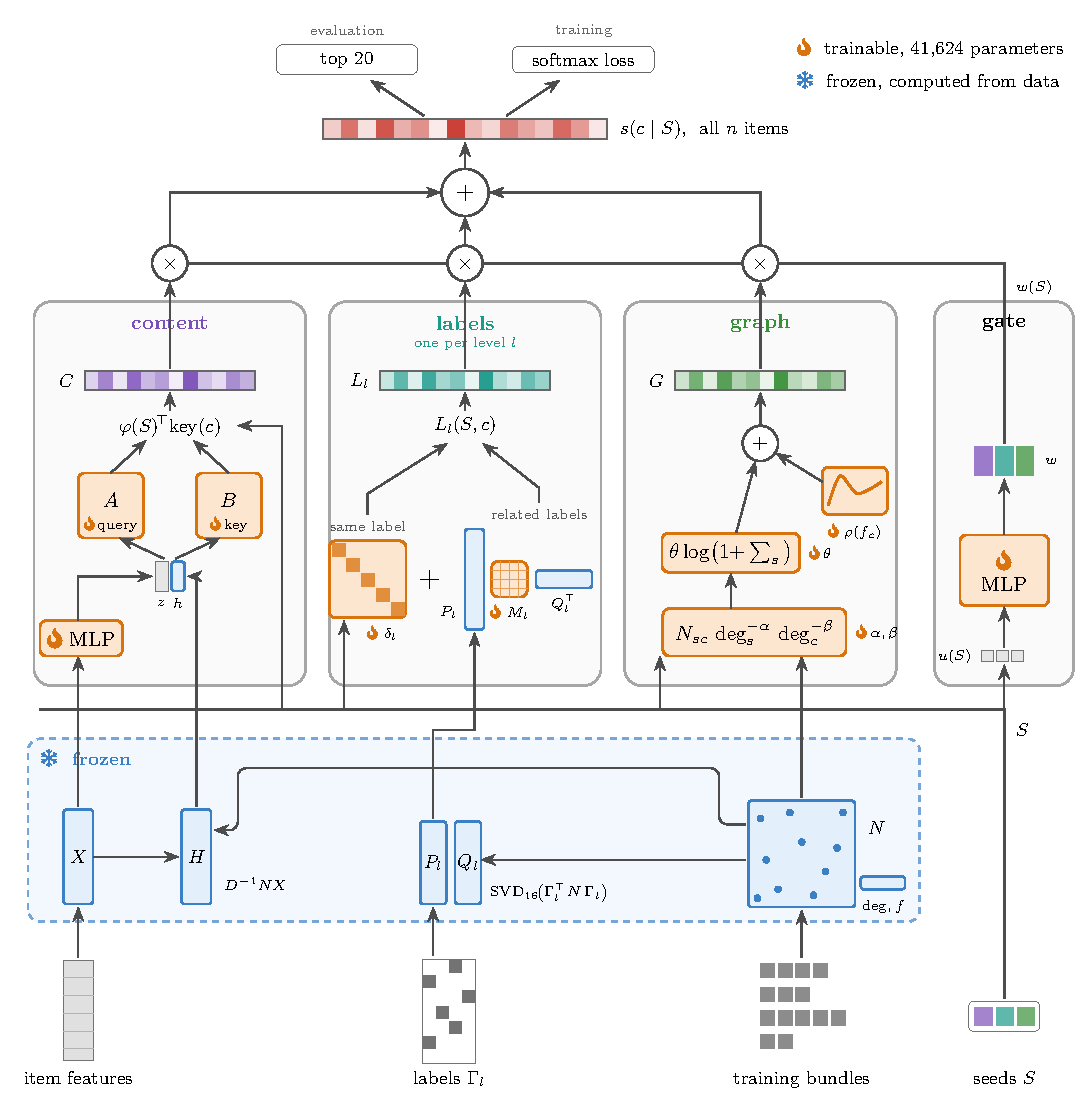
\includegraphics[height=0.85\textheight]{architecture.pdf}
\end{column}
\begin{column}{0.42\textwidth}
\footnotesize
\key{Frozen (blue), from training data:} features $X$, partner history $H=D^{-1}NX$, label factors $P_l,Q_l$ (SVD of $\Gamma_l^\top N\Gamma_l$), counts $N$.\par
\vspace{3mm}
\key{Trained (orange), three terms per item:}
\begin{itemize}\setlength\itemsep{0pt}
\item content: maps $A,B$ of $[z,h]$
\item labels: $\delta_l$ plus $P_lM_lQ_l^\top$
\item graph: damped counts plus prior $\rho(f_c)$
\end{itemize}
\vspace{2mm}
\key{Gate:} reads the seeds, outputs one weight per term.\par
\vspace{3mm}
\key{Output:} $s(c\mid S)$ for all $n$ items; top 20, or softmax loss in training.\par
\vspace{3mm}
\fn{41,624 trained parameters; nothing per item.}
\end{column}
\end{columns}
\end{frame}

% ------------------------------------------------------------------ 7
\begin{frame}{DIALS: the score}
\small
\begin{align*}
 s(c\mid S)=\;&w_C(S)\,\underbrace{\phi(S)^\top\psi(c)}_{\text{content}}\\
 +&\sum_l w_l(S)\Big[\underbrace{\delta_l(\cdot)\,[t_{g(c)}(S)>0]}_{\text{shared label}}+\underbrace{\tfrac{t(S)^\top}{|S|}P_lM_lQ_l^\top e_{g(c)}}_{\text{label relation}}\Big]\\
 +&\;w_G(S)\Big[\underbrace{\theta\log\big(1+\textstyle\sum_{s\in S} n_{sc}\,d_s^{-\alpha}d_c^{-\beta}\big)}_{\text{co-occurrence}}+\underbrace{\rho(f_c)}_{\text{prior}}\Big]
\end{align*}
\vspace{2mm}
\renewcommand{\arraystretch}{1.1}\footnotesize
\begin{adjustbox}{max width=\textwidth}\begin{tabular}{@{}p{0.30\textwidth}p{0.63\textwidth}@{}}
$\phi,\psi$ & rank-64 maps of item features and partner history\\
$\delta_l$ & small MLP; its \key{sign is learned} (substitute vs complement)\\
$P_l,Q_l$ fixed, $M_l$ ($16\times16$) learned & which labels go with which\\
$w(S)=\mathrm{softplus}(\mathrm{MLP}(\cdot))$ & per-query trust in each term\\
\end{tabular}\end{adjustbox}\par
\vspace{3mm}
\key{One configuration on all 8 datasets; no per-item parameters.}
\end{frame}

% ------------------------------------------------------------------ 8
\begin{frame}{Training without leakage}
\begin{enumerate}\setlength\itemsep{8pt}
\item \key{Leave-one-out.} A training bundle is scored with its own contribution removed from every count, degree, frequency and partner history.
\item \key{Cross-fitting.} The label SVD cannot be corrected that way, so a bundle being trained on uses factors computed without its fold (5 folds).
\item \key{Full-catalogue softmax.} Every hidden item competes with all items outside its bundle: no negative sampling.
\end{enumerate}
\vspace{4mm}
\fn{Why it matters: an earlier version with free label embeddings memorized the bundles of rare labels; on Dunnhumby, a user-history term without leave-one-out drove training loss to 5.5 and validation NDCG to .06.}
\end{frame}

% ------------------------------------------------------------------ 9
\begin{frame}{Results: against the best simple baseline}
\centering\renewcommand{\arraystretch}{1.3}\small
\begin{adjustbox}{max width=\textwidth}\begin{tabular}{llrrrr}\toprule
Dataset & Best simple (on validation) & Its N & DIALS N & $\Delta$N [95\% CI] & $p$ (N)\\\midrule
Electronic & content+ItemKNN & .299 & .335 & +.036 [.016,.057] & .002\\
Food & content+ItemKNN & .425 & .439 & +.014 [$-$.006,.034] & \textcolor{Warn}{.28}\\
Clothing & content+ItemKNN & .330 & .388 & +.057 [.035,.080] & .002\\
Dunnhumby & content+ItemKNN & .104 & .102 & \textcolor{Warn}{$-$.002 [$-$.005,.001]} & \textcolor{Warn}{.28}\\
POG\_DENSE & RP3$\beta$ & .241 & .280 & +.040 [.036,.043] & .002\\
POG & EASE & .0198 & .0313 & +.012 [.009,.014] & .002\\
Spotify\_sparse & content+ItemKNN & .153 & .256 & +.104 [.095,.112] & .002\\
Spotify & content+ItemKNN & .223 & .282 & +.060 [.054,.066] & .002\\\bottomrule
\end{tabular}\end{adjustbox}\par
\raggedright\vspace{2mm}
\fn{Clean test queries, 3 seeds, full-catalogue NDCG@20; paired cluster bootstrap, sign-flip test, Holm over 16 tests. Baselines: popularity, co-occurrence, ItemKNN, RP3$\beta$, GF-CF, EASE, iALS, SGFCF, blend.}
\end{frame}

% ------------------------------------------------------------------ 10
\begin{frame}{Results: against CLHE and RaMen, rerun on identical splits and features}
\centering\renewcommand{\arraystretch}{1.3}\small
\begin{adjustbox}{max width=\textwidth}\begin{tabular}{lrrrrr}\toprule
Test NDCG@20 & CLHE & RaMen & \key{DIALS} & $\Delta$ vs best neural & Parameters (CLHE / RaMen / DIALS)\\\midrule
Electronic & .260 & .254 & \textbf{.335} & +.075 & 0.75M / 1.31M / 41.6k\\
Food & .272 & .274 & \textbf{.439} & +.164 & 0.78M / 1.38M / 41.6k\\
Clothing & .186 & .191 & \textbf{.388} & +.197 & 0.88M / 1.56M / 41.6k\\
POG\_DENSE & .248 & & \textbf{.280} & +.033 & 7.25M / 11.6M / 41.6k\\
POG & .0172 & & \textbf{.0313} & +.014 & 9.48M / 16.1M / 41.6k\\
Spotify\_sparse & .115 & & \textbf{.256} & +.141 & 29.0M / 56.5M / 42.0k\\\bottomrule
\end{tabular}\end{adjustbox}\par
\raggedright\vspace{2mm}
\fn{Their own code, 3 seeds each, settings chosen on validation; all 18 tests $p=.002$ (Holm over 20). Published numbers on the same POG/Spotify split files: RaMen POG .0226, Spotify .1882; DIALS (all queries) .0320, .2831. RaMen's e-commerce numbers (R@20 .84) use an unreleased split and a user--item graph that contains the test bundles.}
\end{frame}

% ------------------------------------------------------------------ 11


% ------------------------------------------------------------------ 12
\begin{frame}{Is it just an ensemble? The final step is a sum; the test is what is summed}
\textbf{Test NDCG@20 (clean), 3 seeds}\par\vspace{1mm}
\centering\renewcommand{\arraystretch}{1.2}
\begin{adjustbox}{max width=\textwidth}\begin{tabular}{lrrr}\toprule
& POG\_DENSE & POG & Spotify\_sparse\\\midrule
Standard scorers, tuned weighted sum$^c$ & .249 & .0234 & .205\\
DIALS terms, \key{fixed} weights & .277 & .0308 & .240\\
DIALS terms, \key{per-query gate} & \textbf{.280} & \textbf{.0313} & \textbf{.256}\\\bottomrule
\end{tabular}\end{adjustbox}\par
\raggedright\vspace{2mm}
\begin{itemize}\setlength\itemsep{1pt}\small
\item \key{Same evidence, standard scorers:} the best tuned weighted sum loses .008--.051 to DIALS ($p=.0008$ on all 4 datasets).
\item \key{Same learned terms, fixed weights:} keeps most of the gain. The gain is in the learned terms.
\item \key{The gate adds} +.016 on Spotify\_sparse, +.003 on POG\_DENSE, +.002 on Dunnhumby (Holm $p\le.0014$); not separated on Electronic, Food, Clothing, POG.
\end{itemize}
\fn{$^c$Label rules + ItemKNN + content, weights tuned on validation. Fixed weights = each dataset's mean gate on validation queries; trained model otherwise unchanged; Holm over 14 tests.}
\end{frame}

\begin{frame}{What a fixed ensemble cannot do: the relation changes sign by domain}
\centering\renewcommand{\arraystretch}{1.25}
\begin{tabular}{lrr}\toprule
Dataset & $\delta$: one of 3 seeds shares $c$'s label & Gate weights: content / labels / graph\\\midrule
POG & \textcolor{Warn}{$-$0.16} & 4.2 / \textbf{14.8} / 3.7\\
POG\_DENSE & \textcolor{Warn}{$-$0.31} & 6.0 / \textbf{15.2} / 3.1\\
Food & +1.63 & 1.2 / 1.1 / \textbf{4.7}\\
Clothing & +1.91 & 1.9 / 1.6 / \textbf{6.6}\\
Spotify (artist) & +2.63 & \textbf{3.1} / 1.0 / 1.1\\\bottomrule
\end{tabular}\par
\raggedright\vspace{3mm}
\begin{itemize}\setlength\itemsep{2pt}
\item \key{Outfits:} a shared category is evidence \emph{against} (one item per category). Nothing in the model says this.
\item \key{Playlists and e-commerce bundles:} a shared artist or category is evidence \emph{for}.
\item An ensemble of similarity scorers can only add ``same category'' with a positive weight; DIALS learns the sign, with one configuration on every dataset.
\end{itemize}
\end{frame}

% ------------------------------------------------------------------ 13
\begin{frame}{Why it works: where the lead comes from}
\textbf{Test NDCG@20 by the most co-occurrence any seed has with the target}\par\vspace{2mm}
\centering\renewcommand{\arraystretch}{1.3}
\begin{adjustbox}{max width=\textwidth}\begin{tabular}{llrrrr}\toprule
Dataset & & 0 & 1 & 2--3 & 4+\\\midrule
POG\_DENSE & share of queries & 36\% & 15\% & 14\% & 35\%\\
& CLHE / \key{DIALS} & .137 / \textbf{.151} & .249 / \textbf{.265} & .302 / \textbf{.328} & .339 / \textbf{.400}\\
POG & share of queries & 96\% & 3\% & 1\% & 0.3\%\\
& CLHE / \key{DIALS} & .005 / \textbf{.019} & .271 / .261 & .458 / .556 & .578 / .666\\\bottomrule
\end{tabular}\end{adjustbox}\par
\raggedright\vspace{4mm}
\begin{itemize}\setlength\itemsep{4pt}
\item \key{POG is a no-history problem:} 96\% of queries have no co-occurrence evidence; there DIALS is 4$\times$ CLHE.
\item \key{The gate responds:} on Spotify\_sparse the graph-to-content weight falls from 0.43 to 0.16 as the share of unseen seeds rises.
\end{itemize}
\end{frame}

% ------------------------------------------------------------------ 14
\begin{frame}{What each term contributes (inference-time knockouts)}
\centering\renewcommand{\arraystretch}{1.3}
\begin{adjustbox}{max width=\textwidth}\begin{tabular}{lrrr}\toprule
Test NDCG@20 (clean) & POG\_DENSE & POG & Spotify\_sparse\\\midrule
\key{Full DIALS} & \textbf{.280} & \textbf{.0313} & \textbf{.256}\\
without content & .239 & .0198 & .232\\
without labels & .261 & .0203 & .137\\
\quad without label low-rank only & .274 & .0269 & .256\\
without co-occurrence & .263 & .0239 & .242\\
without prior & .051 & .0161 & .238\\\bottomrule
\end{tabular}\end{adjustbox}\par
\raggedright\vspace{3mm}
\key{Every term matters somewhere, and which one matters most depends on the domain:} the prior on POG\_DENSE, labels on Spotify, content and labels together on POG.\par
\vspace{2mm}\fn{Trained weights kept; nothing retrained. 3 seeds.}
\end{frame}

% ------------------------------------------------------------------ 15
\begin{frame}{Practical value: what DIALS costs to run}
\centering\renewcommand{\arraystretch}{1.35}\small
\begin{adjustbox}{max width=\textwidth}\begin{tabular}{lrrr}\toprule
& \key{DIALS} & CLHE & RaMen\\\midrule
Trained parameters (POG) & \textbf{41.6k} & 9.48M & 16.1M\\
Per-item parameters & \textbf{none} & 2 tables $n\times64$ & 256 per item\\
Training on POG (4 CPU threads) & \textbf{12--15 min} & 85 min & 71 min$^*$\\
Inference, ms/query on CPU (POG / Spotify) & 0.49 / 3.24 & 0.53 / -- & 0.69 / --\\
Full Spotify training & CPU, hours & $\approx$6.5 GPU-h per seed & --\\\bottomrule
\end{tabular}\end{adjustbox}\par
\raggedright\vspace{3mm}
\begin{itemize}\setlength\itemsep{3pt}
\item \key{New items on day one:} scored from features and category, no retraining.
\item \key{Explainable:} each recommendation decomposes into named terms and gate weights.
\item \key{Honest cost:} memory is dominated by the co-occurrence matrix: about 560 MB on Spotify (about 260 MB compressed), against about 130 MB for CLHE and 260 MB for RaMen.
\end{itemize}
\fn{$^*$RaMen: 21 s per epoch measured, times its configured 200 epochs; not trained to completion by us.}
\end{frame}

% ------------------------------------------------------------------ 16
\begin{frame}{Where DIALS does not win}
\begin{itemize}\setlength\itemsep{8pt}
\item \key{Dunnhumby (grocery baskets):} ties the content+ItemKNN blend ($-$.002 NDCG, $p=.28$). Warm and co-occurrence-driven; 97\% of items are in training baskets.
\item \key{Personalization helps everyone equally:} adding the household's repurchase counts lifts DIALS by 45\% (.102 $\to$ .148), and the blend by 42\% (.104 $\to$ .148): a tie again.
\item \key{Food:} recall separated, NDCG not ($p=.28$).
\item \key{Features matter on POG:} the released BLIP text features on Chinese titles cost DIALS 13\% against a Chinese text encoder (.0313 vs .0360).
\item \key{Open:} CLHE on full Spotify has 1 of 3 seeds; RaMen not rerun on POG/Spotify.
\end{itemize}
\end{frame}

% ------------------------------------------------------------------ 17
\begin{frame}{Contribution, stated so it can be defended}
\begin{enumerate}\setlength\itemsep{6pt}
\item \key{Separate, jointly learned evidence terms} (late fusion) instead of one fused item vector; a per-query gate on top, which matters where history varies across queries (+6\% on Spotify\_sparse).
\item \key{Labels as a learned relation:} a signed diagonal (substitute vs complement) plus a low-rank label-to-label map on cross-fitted spectral factors.
\item \key{One configuration} that recovers opposite domain structure (avoid the seed's category on fashion, same artist on music) on 8 datasets.
\item \key{Leakage-free training} by leave-one-out and cross-fitting.
\end{enumerate}
\vspace{1mm}
\fn{The components exist separately (graph filters with degree exponents, category compatibility, homophily/heterophily learning); the claim is the combination and its measured effect, not that any part is first.}\par
\vspace{1.5mm}
\key{In one line:} bundle completion that works without purchase history, with 41.6k parameters.\par
\vspace{1mm}
\key{Next:} Instacart (real product names and aisles); TIFU-KNN and UP-CF@r for the personalized task; RaMen on POG and Spotify.
\end{frame}

% ------------------------------------------------------------------ backup
\begin{frame}{Backup: other published protocols}
\small
\textbf{Bundle-MLLM (KDD'25), HitRate@1 among 10 candidates, released split files:}\par\vspace{1mm}
\centering\renewcommand{\arraystretch}{1.25}
\begin{adjustbox}{max width=\textwidth}\begin{tabular}{lrrr}\toprule
& \key{DIALS} & Bundle-MLLM (published) & CLHE (in that paper)\\\midrule
POG & \textbf{.630} & .413 & .348\\
POG\_DENSE & \textbf{.781} & .668 & .637\\\bottomrule
\end{tabular}\end{adjustbox}\par
\vspace{4mm}\raggedright
\textbf{DDBC (ICLR'26), F1 within a candidate pool:}\par\vspace{1mm}
\centering
\begin{adjustbox}{max width=\textwidth}\begin{tabular}{lrrr}\toprule
& \key{DIALS} & Best simple & DDBC (published)\\\midrule
POG, $k=4$ & \textbf{.488} & .452 & .139\\
Spotify, $k=30$ & \textbf{.625} & .540 & .282\\\bottomrule
\end{tabular}\end{adjustbox}\par
\raggedright\vspace{2mm}
\fn{Published numbers, not rerun. Bundle-MLLM states an 8:1:1 split; only 7:1:2 files are released, and those are used.}
\end{frame}
\end{document}
